\documentclass[12pt]{report}
\usepackage{amsmath}
\usepackage{amssymb}
\usepackage{graphicx}
\usepackage{longtable}

\newcommand{\bt}[1]{\textbf{#1}}
\newcommand{\ubt}[1]{\textbf{\underline{#1}}}
\newcommand{\sps}{\\[0.2cm]}
\newcommand{\spn}[1]{\\[#1cm]}
\newcommand{\refn}[1]{\textbf{(\ref{#1})}}
\newcommand{\NI}{\noindent}
\newcommand{\beq}{\NI$\displaystyle}
\newcommand{\eeq}{$}
\newcommand{\eeqn}{$\\[0.3cm]}
\newcommand{\dsp}{\displaystyle}

\renewcommand*\contentsname{Table of Contents}
\renewcommand{\baselinestretch}{1.5}

\begin{document}
	%%remove the numbering from the first page 
	\clearpage
	\thispagestyle{empty}
	%%TITLE%%
	\addcontentsline{toc}{chapter}{TITLE PAGE}
	\begin{center}
		{\bf \LARGE AN IMPROVED SIR MODEL WITH REALISTIC ASSUMPTION }
	\end{center}
	$$$$
	\begin{center}
		\textbf{\itshape\large BY}
	\end{center} 
	$$$$
	\begin{center}
		{\bf AWOTAYO, ADEDOYIN REUBEN\\
			16/56EB050}
	\end{center}
	$$$$
	\begin{center}
		\textbf{A PROJECT SUBMITTED TO THE
			DEPARTMENT OF MATHEMATICS, FACULTY OF PHYSICAL SCIENCES,
			UNIVERSITY OF ILORIN, ILORIN, NIGERIA,
			$$$$
			IN PARTIAL 
			FULFILMENT OF REQUIREMENTS FOR THE AWARD OF
			BACHELOR OF SCIENCE {\itshape{(B.Sc.)}} DEGREE IN MATHEMATICS.}
	\end{center}
	$$ $$ 
	\\ \\
	\begin{center}
		{\bf JUNE, 2021}
	\end{center}
	\newpage
	\pagenumbering{roman} 
	\addcontentsline{toc}{chapter}{CERTIFICATION}
	\section*{\begin{center}\textbf{\Large CERTIFICATION}   \end{center}}
	This is to certify that this project was carried out by \textbf{AWOTAYO, ADEDOYIN REUBEN} of Matriculation Number  16/56EB050, for the award of Bachelor of Science B.Sc degree in the Department of Mathematics, Faculty of Physical sciences, University of Ilorin, Ilorin, Nigeria.
	\\
	\\
	................................... \qquad \qquad\qquad\qquad\qquad\qquad...................... \\
	PROF. M.S. DADA  \qquad\qquad\qquad\qquad\qquad\qquad\quad Date\\
	(SUPERVISOR)\\
	\\
	\\
	\\
	...................................... \qquad\qquad\qquad\qquad\qquad\qquad ......................\\
	PROF. K. RAUF      \qquad\qquad\qquad\qquad\qquad\qquad\qquad\quad     Date\\
	(HEAD OF DEPARTMENT)\\
	\\
	\\
	\\
	..................................... \qquad\qquad\qquad\qquad\qquad\qquad .......................\\
	PROF. T. O. OLUYO  \qquad\qquad\qquad\qquad\qquad\qquad \quad        Date\\
	(EXTERNAL EXAMINER)
	
	\newpage
	%%DEDICATION%%
	\section*{\begin{center}	\textbf{\Large DEDICATION}   \end{center}}
	\addcontentsline{toc}{chapter}{DEDICATION}
	I would like to dedicate the project to God, for the grace and faithfulness of God thus far. For His mercies, guidance and protection throughout these years of study.
	
	\newpage
	%%ACKNOLEDGEMENT%%
	\section*{\begin{center}\textbf{\Large ACKNOWLEDGMENTS}\end{center}}
	\addcontentsline{toc}{chapter}{ACKNOWLEDGMENTS} 					
	All thanks to God the Almighty, the one who is and will forever be, the one and only true God, for all He was done for me throughout the course of my academic journey in the University of Ilorin. May the name be praised forever.\\
	
	\NI I wish to express my profound gratitude to my Project Supervisor, Prof. M.S. Dada for his efforts and support towards this project. May God bless you and your family Sir.\\
	
	\NI I also want to acknowledge my H.O.D, Prof. K. Rauf, and other lecturers of the department who have contributed in one way or another to my academic success: Prof. J.A Gbadeyan, Prof. T.O. Opoola, Prof. O.M. Bamigbola, Prof. M.O. Ibrahim, Prof. O.A. Taiwo, Prof. R.B. Adeniyi, Prof. K.O. Babalola, Prof. M.S. Dada, Prof. A.S. Idowu, Doctors E.O. Titiloye, O.A. Fadipe-Joseph, Y.O, Aderinto, C.N. Ejieji, B.M. Yisa, J.U. Abubakar, K.A. Bello, G.N. Bakare, B.M. Ahmed, O.T. Olotu, I.F. Usamot, O.A. Uwaheren, O. Odetunde, T.L. Oyekunle, A.A. Yeketi, also the efforts of the non-academics staff of he department, may God reward you all and your families.\\
	
	\NI My eternal and immeasurable gratitude goes to my Mom, Mrs. Awotayo Bamidele Heritage and my Aunt, Mrs. Giwa Elizabeth, they have stood behind me solidly through all. Thank you for your words of advise, encouragement and all the efforts you have put in me to make who I am today, I will be forever be indebted to you both. God bless you abundantly.\\
	
	\NI I want to say a big thank you to all my friends who believed and still believe in me, those who helped me in one way or the other during my academic years in this school. God bless you all.\\
	
	\newpage
	%%ABSTRACT%%
	\section*{\begin{center}\textbf{\Large ABSTRACT}\end{center}}
	\addcontentsline{toc}{chapter}{ABSTRACT}
	David and Lang developed a mathematical model (SIR) i.e. Susceptible - Infective - Recovered for the spread of infectious in a given population over a time. The model gives a reasonable and sound results. However, some more realistic factors have not been accounted for in their model. These realistic assumptions will give better understanding of the modelling epidemics if included. 
	
	%%TABLE OF CONTENTS%%
	\addcontentsline{toc}{chapter}{TABLE OF CONTENTS}
	\tableofcontents
	\newpage
	
	\pagenumbering{arabic}
	%%%%%%%%%%%%%%%%%%%%%%%%%CHAPTER ONE%%%%%%%%%%%%%%%%%%%%%%%%%%%%
	\chapter{INTRODUCTION TO MATHEMATICAL MODELING}
	Mathematical Modeling is the art of translating problems from an application area into tractable mathematical formulations whose theoretical and numerical analysis provides insight, answers, and guidance useful for the originating application (Tymoczko, 2011).\\
	
	\NI Mathematical Modeling
	\begin{itemize}
		\item is indispensable in many applications
		\item is successful in many further applications
		\item gives precision and direction for problem solution
		\item enables a thorough understanding of the system modeled
		\item prepares the way for better design or control of a system
		\item allows the efficient use of modern computing capabilities
	\end{itemize}
	
	\section{ELEMENTS OF MATHEMATICAL MODEL}
	Mathematical models can take many forms, including dynamical systems, statistical models, differential equations, or game theoretic models. These and other types of models can overlap, with a given model involving a variety of abstract structures (Billings, 2013).\\
	
	\NI In Physical Sciences, a mathematical model contains most of the following elements:
	\begin{enumerate}
		\item Governing equations
		\item Suplimentary sub-models
			\begin{itemize}
				\item Defining equations
				\item Constitutive equations
			\end{itemize}
		\item Assumptions and Constants
			\begin{itemize}
				\item Initial and boundary conditions
				\item Classical constraints and kinematic equations
			\end{itemize}
	\end{enumerate}
	\newpage
	\section{LIST OF APPLICATION}
	\begin{itemize}
		\item Anthropology
			\begin{itemize}
				\item Modeling, classifying and reconstructing skills
			\end{itemize}
		
		\item Archaeology 
			\begin{itemize}
				\item Reconstruction  of objects fro preserved fragments
				\item classifying ancient artifices
			\end{itemize}
		
		\item Architecture
			\begin{itemize}
				\item Virtual Intelligence
			\end{itemize}
		\item Artificial Intelligence
		\item Arts
		\item Astronomy
		\item Biology
			\begin{itemize}
				\item Protein folding
				\item Humane genome project
				\item population dynamics
				\item Morpho genesis
				\item Evolutionary pedigree
				\item Spreading of infections diseases
				\item Animal and plant breeding (genetic variability)
			\end{itemize}
		
		\item Chemical Engineering
		\item Chemistry
		\item Computer Science etc
	\end{itemize}

	\section{BASIC NUMERICAL TASKS}
	The following is a list of categories containing the basic algorithmic toolkit needed for extracting numerical information from mathematical models.
	\begin{enumerate}
		\item Numerical Models
		\begin{itemize}
			\item Linear systems of equations, Eigen value problems, Linear programming (Linear optimization), Techniques for larege sparse problems
		\end{itemize}
	
		\item Numerical Analysis
		\begin{itemize}
			\item Function evaluation, Automatic and Numerical differentiation, interpolation, Approximation(Padi, lease square, radial basis, functions), Interpolation(univariate, multivariate, fourier transform), special functions, Non-linear systems of equations, optimization, technique for large, sparse problems.
		\end{itemize}
		
		\item Numerical data analysis (Numerical statistics)
		\begin{itemize}
			\item Visualization(2D and 3D computational geometry), parameter estimation(least squares, maximum likelihood), prediction, classification, Time series analysis (signal processing, filtering, time correlations, spectral analysis), categorical time series(hidden Markov models), Randoms numbers and Monte Carlo methods.
		\end{itemize}
	
		\item Numerical functional analysis
		\begin{itemize}
			\item Ordinary differential equations(initial value problems, boundary value problems, eigen value problems, stability), techniques for large problems, partial differential equations (finite differences, finite elements, boundary elements, mesh generation, adaptive meshes), stochastic differential equation, integral equation (and regularization)
		\end{itemize}
	
		\item Non-numerical Algorithms
		\begin{itemize}
			\item Symbolic methods (computer algebra), sorting, compression, cryptography (\textit{http://www.mat.univie.ac.at/\~neum/})
		\end{itemize}
	\end{enumerate}


	\section{EXAMPLES OF MATHEMATICAL MODELING}
	Having talked about mathematical modeling and its relation to real world and mathematical worlds
	\begin{enumerate}
		\item Model of blood flow
		\item model of drug dosage
		\item model of yellow fever
		\item model of rocket flight and implication
		\item model of population growth
		\item oil reservoir model
		\item model of HIV
		\item model of simple pendulum neglecting air resistance and friction at the pivot
		\item model of Epidemic
		\item model of chicken pox
		\item model of Ebola (Oluniyi, 2017)
	\end{enumerate}

	\section{STEPS IN BUILDING A MATHEMATICAL MODEL}
	\bt{STEP 1: Understand the concepts of the application area} \\
	Before we can build a mathematical model, we must first understand the concepts needed from the application area where answers to specific questions are desired. Solution of the model should provide answers to these questions. We start with a description of the phenomenon to be molded, including the 'laws' you must follow (e.g that are imposed by nature, by an entrepreneurial environment or by the modeler). The need to answer questions about brain tumor will drive us to medical biology.\\
	\newpage
	\NI\bt{STEP 2: Understand the mathematical concept needed}\\
	In order to develop and solve a mathematical model, we must first be sure we know the appropriate mathematics.\spn{0.4}
	To understand Mathematical concepts needed for the particular model, you have to be reasonably proficient in high school algebra including how to solve algebraic equations and including how to compute derivatives and anti-derivatives. We are developing the required techniques and understanding of differential equations.\\
	
	\NI Additional required mathematics after first order ODE's (and solution of second order ODE's by first order techniques) is linear Algebra. All of these must be mastered in order to understand the development and solution of mathematical models in science and engineering.\\
	
	\NI\bt{STEP 3: Develop the mathematical model}\\
	The model must include those aspects of the application so that its solution will provide answers to the questions of interest. However, inclusion of two much complexity may make the model unsolvable and useless. To develop the mathematical model, we use laws that must be followed, diagrams we have drawn to understand the process and notation and nomenclature we developed. Investigation of these laws results in a mathematical model. Please note here that a mathematical model for example that deals with Brain Tumor, must be mentally, Biologically and Mathematically correct.\spn{0.6}
	
	\NI\bt{STEP 4: Solve the mathematical model}\\
	Once correctly formulated, the solver of the mathematical model can rely completely on mathematics and need not know where the model came from or what the nomenclature stands for solution of the model requires both practical ("how to") skills and theoretical ("why") skills.\spn{0.4}
	For a general linear autonomous model, we can obtain a general formula for its uniqueness. If specific data is given, we can insert it into our formula.\\
	
	\NI\bt{STEP 5: Interpretation of results}\\
	Although interpretation of results can involve lots of things, in the current context where the general model has been solved, it means insert the specific data given in the problem into the formula and answer the questions asked with regard to that specific data. This may require additional solution of algebraic equation (Oluniyi, 2017).\\
	
	\section{CLASSIFICATION OF MODELS AND PROBLEMS}
	\begin{enumerate}
		\item \bt{Static Vs Dynamic Models}\\
		Static models are at equilibrium or steady state, at opposed to dynamic models when change with respect to time.\spn{0.4}
		
		\item \bt{Deterministic Vs Stochastic Models}\\
		Deterministic models have no components that are inherently uncertain, i.e no parameters in the model  are characterized by probability distribution, as opposed to stochastic models. For fixed starting values, a deterministic model will always produce the same result. A stochastic model will produce many different results depending on the actual value that the random variables take in each realization.
		
		\item \bt{Continuous Vs Discrete Models, Differential Vs Difference equation}
		
		\item \bt{Individual Vs Structured Models}\\
		Structured models based on age, size, stage etc.
		
		\item \bt{Mechanistic Vs Statistical Models}\\
		Statistical or Empirical models are usually regression based. They provide a quantitative summary of the observed relationships among a set of measured variables. A mechanistic or Scientific model begins with a description of how nature might work, and proceeds from description to a set of predictions relating to the independent and dependent variables.
		
		\item \bt{Qualitative Vs Quantitative Models}\\
		Qualitative models lead to a detailed, numerical prediction about responses, whereas qualitative models lead to general descriptions about the responses (Li et al., 2018).
	\end{enumerate}

	\chapter{LITERATURE REVIEW}
	Malaria, AIDS, and Cholera are only a few of the infections diseases that continue to claim millions of lives around the world (Busenberg S. Cooke, 1993). Infection eradication efforts around the world, on the other hand, have a long way to go.\spn{0.5}
	For several years, illnesses have been introduced with a significant achievement (Howard Weiss, 2013). He goes on to illustrate how the paradigm aids in the comprehension of a theoretical study for programs in public health\spn{0.5}
	The use of mathematical modeling to predict the spread of epidemics has a long way history, beginning Daniel Bernoulli's research on the effects of cow-pox vaccination. In 1760 on the spread of smallpox (Keelng, Woolhouse, Davies and Greepfell(2003)) cite a number of examples. Diseases are all  around us. Many, such as the common cold, have been around for a long time. Others, such as mild symptoms, are merely an annoyance; however, others such as viruses like Ebola and Aids make us afraid. Through the dawn of time to the present. Diseases today are a cause of anxiety and superstition.\\
	
	\NI Meghan (1998) invented a basic mathematical model for estimating the number of people infected with a disease like chicken pox in a closed population. His research revealed that if the parameter controlling disease distribution is positive, the disease would spread throughout the population, making eradication impossible. The chicken pox, on the other hand, dies out in the population if the parameter is negative. In epidemics such as cholera and bubonic plague in London, Kermack and Mckendrick (1927) suggested a SIR model to explain the rapid rise and fall in the number of infected patients. They assumed a fixed population size, that infectious agent incubation is instantaneous, and that infectivity lasts for the same amount of time as the length of the infection. An outbreak will occur, according to the report if and only if the initial susceptible fraction is greater than the rationing for reproduction ($R_O$).\\
	
	\NI Troy (2005) used David and Lang's data to develop a statistical model that explains "excess" pneumonia influenza deaths (2001). He presumed that, in a predetermined situation, homogeneous group of people, excess deaths are on the rise proportional to the number of cases of the disease over a period of time the span of time. The research revealed that if $R_0 < 1$, the disease would be eradicated with the passing of time.\\
	
	\NI Keeling (2001) calculated the reproductive ratio ($R_0$) of a number of species; malaria $R_0 \approx 100$, measles $R_0 \approx 18$, small pox $R_0 \approx 4$ and AIDS $R_0 \approx 5$. His investigation showed that, infectious diseases with high values $R_0$ are harder to monitor than those with lower values of $R_0$.\\
	
	\NI Brockmann and Geisel (2003) created a probalistic model based on the mathematical model (SIR) to explain the global spread of infectious diseases such as Severe Acute Respiratory Syndrome (SARS) which affects the lungs. The model blends a stochastic local infection dynamics with a global infection dynamics. The model was used to forecast the spread of the disease for ninety days fate, the initial outbreak in Honk Kong 2003.\\
	
	\NI The simulations findings were strikingly similar to the global spread of SARS as stated by the World Health Organization (WHO).\\
	
	\NI The mathematical model (SIR) for the spread of infectious diseases such as Hong Kong flue in New York was created by David and Lang (2001). The total population is believed to be set by ignoring births, immigration, and deaths during the epidemic. Non-flu-related deaths were also believed to be entirely absent, also they assumed a completely homogeneous population with no age spatial or social structure.\\
	
	\NI According to their findings, if the contact number of the outbreak is small enough, there would be no epidemic, and vice versa.\\
	\newpage
	\NI The existing model\\
	The existing SIR model is given as\\
	\begin{eqnarray*}
		S' &=& -gS(t), \quad S(0) = S_0 \\
		I' &=& (gS(t) - k), \quad I(0) = I_0\\
		R' &=& kI(t), R(0) = R_0 \text{ where} \spn{0.6}
		S(t) &=& \text{ number of susceptible at time t}\\
		I(t) &=& \text{ number of infected at time t}\\
		R(t) &=& \text{ number of recovered at time t}\\
		N(t) &=& \text{ total population at time t}\\
		g &=& \text{ infectious rate of the disease}\\
		k &=& \text{ recovery rate of the disease}\\
		R_0 &=& \text{ reproductive ratio of the disease}\\
	\end{eqnarray*} 

	\NI The model described in this project is a SIR model in essence. This model divides people into three categories:
	\begin{enumerate}
		\item Susceptible
		\item Infective
		\item Recovered
	\end{enumerate}
	\newpage
	\NI However, in this project, an individual can switch from a susceptible pool to an infected pool when he/she meets an infected person. For instance, catching a common cold may be as simple as walking around the neighborhood, a few feet away from an infected person who has coughed recently. individuals infected with the disease transmit it to those who are susceptible for a period of time in the infectious pool (IJEAS, 2019).
   
   
   \chapter{METHODOLOGY}
   The mathematical modeling approach used to create the new model was modified from the origin SIR model by adding more practical assumptions. The new SIR model is useful for studying infectious diseases, but it isn't flawless. The model would perform better if more practical variables are used.Analysis of the model's equilibrum and stability are going to be investigated.The improved model's eigen values have been investigated. The model's numerical scheme would be introduced and a simulation corresponding to it will be generated,executed in order to chat any interpretations.\\
   
   \NI We consider how certain groups evolve over time and make further assumptions in order to formulate the model. When a susceptible person becomes infected with a high probability of spreading and traveling from susceptible class to the infected class. In a unit of time, all persons that become infected in that unit of time reduce the susceptible  population. Simultaneously, The class of the number of newly infected persons rises by the same amount. The number of individuals who become infected per unit of time in epidemology is called incidence , and the rate of change of the susceptible class is given by $S(t)$=-incidence (Truesdell and Clifford, 1984).\\
   
   \section{MODEL FORMATION}  
   Firstly, we identify the independent and dependent variables. The independent variable is time $(t)$, measured in days, months or years depending on the disease being studied while dependent variables counts people in each of the groups, each as a function of time where
   \begin{eqnarray*}
   	I &=&I(t), \; \text{ number of infected individuals at time $t$}\\
   	S &=&S(t), \; \text{ number of susceptible individuals at time $t$}\\
   	R &=& R(t), \; \text{number of recovery individuals at time $t$ and}\\
   	N &=&N(t), \; \text{ total population at time $t$}\\
   \end{eqnarray*}
   Each individual in a population is in one of the 3 pools.\\
   Thus, $S(t) + R(t) + I(t) = N(t)$\\
   
   \section{ASSUMPTION OF THE MODEL}
   In order to build a more realistic model, we make assumptions in addition to the assumption in David and Lang. Basic SIR models make the following assumptions:
   \begin{enumerate}
   	\item The rate at which the susceptible becomes infected is proportional to the infective and susceptible i.e $gS(t)I(t) >0$ is a constant parameter 
   	
   	\item The rate of recruitment of infective to the recovered pool is proportional to the infective that acquired good treatment $kI(t), k>0$ is a constant parameter.
   	
   	\item The disease is instantaneous (incubation period)
   	
   	\item Birth rate $b>0$, death rate due to natural causes $d>0$
   	
   	\item New borns are born into the susceptible pool and all individuals are to die naturally in any population pool.
   	
   	\item Death of infected individuals is $q>0$ due to the disease.
  
   \end{enumerate}
	
	\section{MODIFIED MODEL}
	The modified model consists of a system of three first order ordinary differential equations that specify the rate of change of three categories of individuals in the population over time.
	\begin{equation}
		S' = b - (gI(t) + d)S(t) \tag{1.1}
	\end{equation}
   \begin{equation}
   	I' = (gS(t) - k - d - q)I(t) \tag{1.2}
   \end{equation}
	\begin{equation}
		R' = kI(t) - dR(t), R(0) = R_0 \tag{1.3}
	\end{equation}
	Each of the differential equation above is given an initial value , so to complete the model,
   
   \begin{equation}
   	S' = b - (gI(t) + d)S(t), s(0)=S_0 \tag{1.4}
   \end{equation}
    \begin{equation}
  	I' = (gS(t) - k - d - q)I(t), I(0)=I_0 \tag{1.5} \label{eq:1_5}
  \end{equation}
  	\begin{equation}
  	R' = kI(t) - dR(t), R(0) = R_0 \tag{1.6}
  \end{equation}
	Where
	\begin{eqnarray*}
	      &b&=\text{ Constant recruitment rate into the susceptible population}\\
	      &d&=\text{ natural death rate of the population}\\ 
	      &q&=\text{ reproductive ratio of the disease.}
    \end{eqnarray*} 
       $\dsp S(t)= \frac {S(t)}{N(t)} ,\quad i(t)=\frac{I(t)}{N(t)},\quad r(t)=\frac{r(t)}{N(t)}$\spn{0.6}
 	And $\dsp S(t) + i(t) + r(t)=1$
 
	 \subsubsection{REPRODUCTIVE RATIO}
	 From \refn{eq:1_5}, It follows that \\
	 $\frac{dI}{dt}=I(gs-k-d-q).$ \\
	 To eradicate the disease in the host population, The condition $\frac{dI}{dt}<0$ must hold implies that\quad $I(gs-k-d-q)<0$ \\
	 Therefore,\quad $ 1<0$ or $(gs-k-d-q)<0 $\\
	 $I<0$ is trivial for epidemic not to occur (eradication)\\
	 Now\\
	 $\dsp(gS-k-q) < 0 \quad \therefore\quad \frac{gS}{k+d+a} < 1$\spn{0.6}
	 Let $R_0 =$ Reproduction ratio\\
	 $\left.\right.\qquad S_0 =$ Initial value of the susceptible population\spn{0.5}
	 $\dsp R_0 =\frac{gS_0}{k+d+q}$\spn{0.7}
	 $R_0$ is the fundamental parameter governing disease dynamics in our model results
	 \begin{enumerate}
	 	\item $R_0 < 1$ physically interpreted to mean one person who gets the disease will infect $<$ 1 person before recovering or dying so the disease will die out and eradication is possible. $\dsp \frac{dI}{dt} < 0$\\
	 	
	 	\item $R_0 > 1$ means each person who gets the disease will infect more than 1 person so the disease will spread in the host population $\dsp \frac{dI}{dt} > 0$\\
	 \end{enumerate}
	  i.e
	  \begin{center}
	  	\begin{figure}[h!]
	  		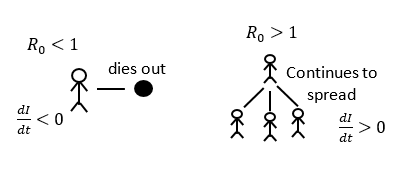
\includegraphics[]{d_c.png}
	  	\end{figure}
	  \end{center}
  
	  \section{STABILITY ANALYSIS OF THE MODEL}
	  We use Jacobian matrix to determine the stability points of the modified model,  obtaining and evaluating at the equilibrium points. The eigen values is determined and is the stability points of the model  
  
	\section{ASYMPTOTIC STABILITY}
	 Considering the modified model equations, we can rewrite as
	 \begin{equation}
	  	S' = b - g(I(t) +d)S(t) = f_1 \nonumber
	 \end{equation}
	\begin{equation}
		I' = g(S(t) - k-d-q)I(t) = f_2 \tag{*} \label{eq:ast}
	\end{equation}
	\begin{equation}
		R' = kI(t) - dR(t) = f_3 \nonumber
	\end{equation}
	Where $f$= incidence rates and are monotonic, concave with respect to $I$ to achieve threshold dynamics of epidemic models.
	
	\section{EQUILIBRIUM OF THE MODEL}
	To evaluate the equilibrium points of the model, the RHS of \bt{(*)} = 0\\
	i.e\\
	\begin{eqnarray*}
		S' &=& b-g(I(t)+d)S(t) = 0\\
		I' &=& g(S(t)-k-d-q)I(t) = 0\\
		K' &=& kI(t) - dR(t) = 0
	\end{eqnarray*}
	Considering $g(S(t) - k-d-q) = 0$, either $I=0$ or $g(S(t)-k-d-q)=0$\\
	However if $\dsp I=0, b-ds=0 \implies S=\frac{b}{d}$\\
	considering $kI(t) - dR(t)$ (if $I=0$), $-dR=0$\\
	$\therefore$ The equilibrium points of the model are $\dsp (\frac{b}{d}, 0,0)$ which is the Disease Free Equilibrium (DFE) \\
	
	\NI\bt{THE JACOBIAN MATRIX}\spn{0.7}
	$J = \begin{bmatrix}
		\frac{\partial f_1}{\partial S} & \frac{\partial f_1}{\partial I} & \frac{\partial f_1}{\partial R}\\
		\frac{\partial f_2}{\partial S} & \frac{\partial f_2}{\partial I} & \frac{\partial f_2}{\partial R}\\
		\frac{\partial f_3}{\partial S} & \frac{\partial f_3}{\partial I} & \frac{\partial f_3}{\partial R}\\
	\end{bmatrix}$
	$\qquad\therefore
	\qquad J = \begin{bmatrix}
		-(gI+d) & -gs & 0\\
		gI & gS-(k+d+q) & 0 \\
		0 & k & -d
	\end{bmatrix}
	$
	\spn{0.7}
	The Jacobian evaluate at the DFE is obtained as\spn{0.5}
	$\dsp J\left(\frac{b}{d},0,0\right) = 
		\begin{bmatrix}
			-d & -\frac{bg}{d} & 0\\
			0 & \frac{bg - (k+d+q)d - \lambda d)}{d} & 0\\
			0 & k & -d
		\end{bmatrix}
	$\spn{0.8}
	THE EIGENVALUES\\
	Using $|J - \lambda I| = 0$\\
	$\lambda_1 =\lambda_2 = -d$ and $\dsp\lambda_3 = \frac{bg-(kd+q)d}{d}$\\
	$\lambda_1$ \& $\lambda_2$ satisfy the negativity requirement for stability because $d$ is a positive parameter\spn{0.3}
	for $\lambda_3 < 0, bg-(k+d+q)d$ must be less than zero since $d>0$. Thus $bg < (k+d+q)d$ which gives $\dsp g < \frac{(k+d+q)}{b}$\spn{0.5}
	
	\NI Therefore, the DFE is totally asymptotically stable, hence the disease eradication is possible under these conditions.
	
	\section{NUMERICAL SCHEME FOR THE MODEL EQUATIONS}
	Considering the system of first order ODE\\
	\begin{eqnarray*}
		S_{n+1} &=& S_n(I-h(gI_n+d)) + hb, S(0)=S_0\\
		I_{n+1} &=& I_n(I+h(gS_n-k-d-q)), I(0) = I_0\\
		R_{n+1} &=& R_n(I-dh) + hKI_n, R(0)=R_0 \quad\text{ for } n=0,1,2,\ldots
	\end{eqnarray*}
	Differential equations that arise from the formulation of our model can be written as\\
	\begin{equation}
		S' = b - (gI +d)S, S(0)= S_0\qquad \nonumber
	\end{equation}
	\begin{equation}
		I' = (gS - K -d-q)I, I(0) = S_0 \nonumber
	\end{equation}
	\begin{equation}
		R' = kI - dR, R(0) = R_0\qquad\qquad \tag{**} \label{eq:astt}
	\end{equation}
	Using Euler's formula, we can write the system of equilibrium as
	\begin{eqnarray*}
		S_{n+1} &=& S_n + h(S')_n\\
		I_{n+1} &=& I_n + h(I')_n\\
		R_{n+1} &=& R_n + h(R')_n\\
	\end{eqnarray*}
	From \bt{(**)} we have\\
	\begin{eqnarray*}
		(S')_n &=& b-(gI_n + d)S_n\\
		(I')_n &=& (gS_n - k-d-q)I_n\\
		(R')_n &=& kI_n - dR_n \text{ for } n=0,1,2,\ldots
	\end{eqnarray*}
	Substituting, we have
	\begin{eqnarray*}
		S_{n+1} &=& S_n + h(b-(gI_n+d))S_n, S(0)=S_0\\
		I_{n+1} &=& I_n + h(gS_n - k-d-q)I_n, I(0) = I_0\\
		R_{n+1} &=& R_n + h(kI_n - dR_n), R(0)=R_0, \text{ for  } n=0,1,2,\ldots
	\end{eqnarray*}


	\chapter{APPLICATION OF IMPROVED SIR MODEL FOR THE SPREAD OF TYPE A INFLUENZA (H3N2)}
	Type A Influenza $(H3N2)$ cases from CDC 2004 - 2005.\\
	
	\NI Infected cases from 157,759 samples tested from people with flu-like symptoms. 
	\begin{longtable}{|@{\hskip 0.2in}c@{\hskip 0.2in}|@{\hskip 0.2in}c@{\hskip 0.2in}|@{\hskip 0.2in}c@{\hskip 0.2in}|@{\hskip 0.2in}c@{\hskip 0.2in}|@{\hskip 0.2in}c@{\hskip 0.2in}|@{\hskip 0.2in}c@{\hskip 0.2in}|@{\hskip 0.2in}c@{\hskip 0.2in}|c@{\hskip 0.2in}|}
		\hline
		n(wk) & $I_n$ & n(Wk) & $I_n$ & n(Wk) & $I_n$ & n(Wk) & $I_n$ \\ \hline
		0 & 3 & 13 & 675 & 25 & 164 & 37 & 1 \\ \hline 
		1 & 2 & 14 & 580 & 26 & 94 & 38 & 6 \\ \hline
		2 & 7 & 15 & 844 & 27 & 37 & 39 & 0 \\ \hline
		3 & 12 & 16 & 974 & 28 & 26 & 40 & 0 \\ \hline
		4 & 9 & 17 & 1096 & 29 & 15 & 41 & 1 \\ \hline
		5 & 10 & 18 & 1354 & 30 & 8 & 42 & 0 \\ \hline
		6 & 27 & 19 & 1335 & 31 & 5 & 43 & 0 \\ \hline
		7 & 21 & 20 & 1109 & 32 & 3 & 44 & 0 \\ \hline
		8 & 36 & 21 & 936 & 33 & 1 & 45 & 1 \\ \hline
		9 & 63 & 22 & 627 & 34 & 2 & 46 & 0 \\ \hline
		10 & 108 & 23 & 476 & 35 & 0 & 47 & 3 \\ \hline
		11 & 255 & 24 & 295 & 36 & 2 & 48 & 0 \\ \hline
		12 & 472 & & & & & & \\ \hline
		\caption{n=0 is last week in September, beginning of the flu season}
		\label{tb:4_1}	
	\end{longtable}
	\section{SIR MODEL}
	Influenza is a disease that satisfies conditions for an SIR model.
	\begin{itemize}
		\item[-] Population is divided into Susceptible, Infected and Recovered (or Removed) individuals.
		
		\item[-] New strains of influenza make most people Susceptible $(S_n)$ at the beginning of an outbreak.
		
		\item[-] Exposed individuals become infected $(I_n)$ - contact with sputum of infected individuals.
		
		\item[-] Individuals, who recover, enter the recovered group $(R_n)$.
		
		\item[-] Recovered individuals have immunity preventing reinfection.
		
		\item[-] Influenza needs to mutate to be able to attack humans in the next year, as the available susceptibles is small after an influenza outbreak (Joseph M., 2018).
	\end{itemize}
	
	\NI Assuming human population is constant $N$ for the duration of the model simulation,
	\begin{equation*}
		N = S_n + I_n + R_n \qquad \text{ or }\qquad R_n = N-S_n-I_n
	\end{equation*}
	So births and deaths are ignored.\sps
	
	\NI A discrete model is presented for the weekly evolution of the disease.\sps 
	\begin{itemize}
		\item[-] New infected, $I_{n+1}$, result from contact between the Susceptible, $S_n$, and infected, $I_n$, with contact rate $\beta/N$.
		
		\item[-] Infected are cured at a rate proportional to the number of infected, $\gamma I_n$, which becomes recovered, $R_n$.
	\end{itemize}
	The assumptions on contact and cure rates give the SIR model, with the constant population assumption, $N=S_n + I_n + R_n$: 
	\begin{eqnarray}
		S_{n+1} &=& S_n - \frac{\beta}{N}S_nI_n\notag\\
		I_{n+1} &=& I_n + \frac{\beta}{N}S_nI_n - \gamma I_n, \notag\\
		R_{n+1} &=& R_n + \gamma I_n\notag
	\end{eqnarray}
	NOTE: The first two equations have no dependence on $R_n$.\sps
	$\dsp \frac{\beta}{N}S_n$ represented proportion of contacts by an infected individual that result in the infection of a susceptible individual.\sps
	$\gamma$ is the probability that an infected person recovers(enters class $R$ of the SIR model).\sps
	Ratio $\dsp \frac{1}{\gamma}$ is the average length of the infections period of the disease.\sps
	The parameter, $\beta$, reflects the average number of Susceptible contacts an infected will have during the infection (Joseph M., 2018).\sps
	
	\NI The graphs below show the fit to the CDS data and the behaviour of the model\\	
	\begin{center}
		\begin{figure}[!hbt]
			\begin{minipage}[c]{0.5\linewidth}
				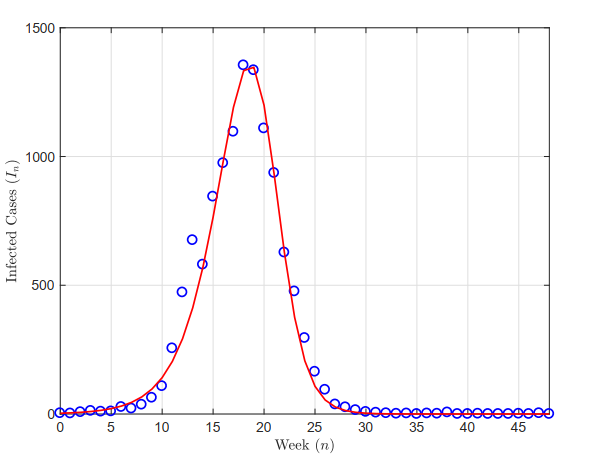
\includegraphics[width=2.8in]{s_m1}
			\end{minipage}
			\begin{minipage}[c]{0.5\linewidth}
				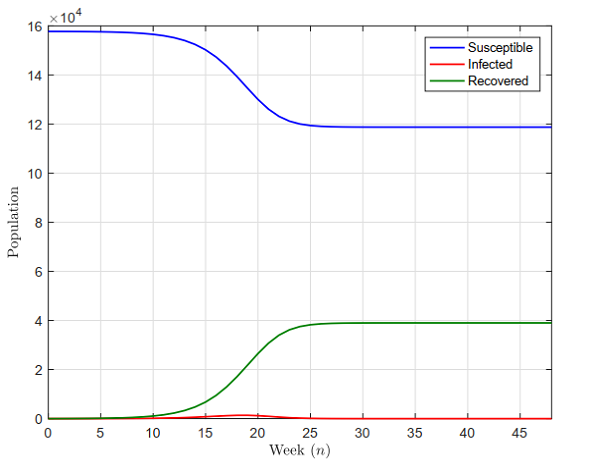
\includegraphics[width=2.7in]{s_m2}
			\end{minipage}
		\end{figure}
	\end{center}
	\NI As the data shows there is a peak on the disease, then it dies off almost as rapidly as it starts.\sps
	The simulation shows that over 48 weeks about 3900 cases of the flu occur, which is about 24.7\% of the population.\sps
	The basic Reproduction Ratio, $R_0$,\\
	\begin{equation*}
		R_0 = \frac{\beta}{\gamma}
	\end{equation*}
	Thus time is $\dsp \frac{1}{\gamma}$, which is about 1.99 days of our case.
	
	\section{SIMULATION OF SIR MODEL FOR INFLUENZA}
	A least squares best fit to the infected population, $I_n$, is fit to the CDC data for the 2004-2005 flu season.
	\begin{eqnarray}
		S_{n+1} &=& S_n - \frac{\beta}{N}S_nI_n\notag\\
		I_{n+1} &=& I_n + \frac{\beta}{N}S_nI_n - \gamma I_n\notag
	\end{eqnarray}
	The model is initialised with $N=157,759, S_0=157,756,$ and $I_0=3$ and run for $n=48$ weeks.\sps
	The SSE is minimised giving
	\begin{equation*}
		\beta = 3.9928 \qquad \text{ and } \gamma=3.5170,
	\end{equation*}
	where SSE = 155,083\sps
	For the CDC case study of the 2004-2005 flue season, our best fitting model give:
	\begin{equation*}
		R_0 \frac{3.9928}{3.5170} = 1.135
	\end{equation*}
	The larger the value of $R_0$, the more infectious the disease.\sps
	
	\NI In the case of Influenza, $R_0$ is only a bit more than 1, which is why survival of the influenza virus depends on its high mutation rate.\sps
	
	\subsection{EQUILIBRIA}
	The SIR model(with constant population $N$) satisfies the equations:
	\begin{eqnarray}
		S_{n+1} &=& S_n - \frac{\beta}{N}S_nI_n,\notag\sps
		I_{n+1} &=& I_n + \frac{\beta}{N}S_nI_n - \gamma I_n\notag
	\end{eqnarray}
	By setting $S_{n+1} = S_n = S_e$ and $I_{n+1}=I_n$ and $I_e$, the first equation satisfies:
	\begin{equation*}
		S_e = S_e - \frac{\beta}{N}S_eI_e, \quad \text{ or } \quad \frac{\beta}{N}S_eI_e = 0,
	\end{equation*}
	which gives $S_e = 0$ or $I_e = 0$.\sps
	The second equation satisfies:
	\begin{equation*}
		I_e = I_e + \frac{\beta}{N}S_eI_e - \gamma I_e, \quad \text{or}\quad \frac{\beta}{N}S_eI_e = \gamma I_e.
	\end{equation*}
	From the second equation:
	\begin{equation*}
		\frac{\beta}{N}S_eI_e = \gamma I_e,
	\end{equation*}
	So, if $S_e=0$, then necessarily $I_e=0$. However, if $I_e =0$, then $S_e$ could be anything.\sps
	It follows that the equlibria are:
	\begin{equation*}
		I_e=0 \quad \text{and}\quad 0 \leq S_e \leq N.
	\end{equation*}
	Thus, the infection must fall to zero, while the Susceptible population could be anything.\sps
	
	\NI The remainder of the population is in the recovered group of individuals.\sps
	
	\section{LINEARIZING ABOUT THE EQUILIBRIA}
	The system
	\begin{equation*}
		\begin{pmatrix}
			S_{n+1}\\
			I_{n+1}
		\end{pmatrix} \quad=\quad
		\begin{pmatrix}
			F(S_n, I_n) \\
			G(S_n, I_n)
		\end{pmatrix}\quad=\quad
		\begin{pmatrix}
			S_n - \frac{\beta}{N}S_nI_n\\
			(1-\gamma)I_n + \frac{\beta}{N}S_nI_n
		\end{pmatrix}
	\end{equation*}
	is linearised using the Jacobian matrix, which satisfies:
	\begin{equation*}
		J(S_n, I_n) = 
			\begin{pmatrix}
				\dsp\frac{\partial F}{\partial S_n} & \dsp\frac{\partial F}{\partial I_n}\spn{0.5}
				\dsp\frac{\partial G}{\partial S_n} & \dsp\frac{\partial G}{\partial I_n}
			\end{pmatrix}
			=
			\begin{pmatrix}
				\dsp 1 - \frac{\beta}{N}I_n & -\dsp\frac{\beta}{N}S_n\spn{0.5}
				\dsp\frac{\beta}{N}I_n & 1 - \dsp\gamma+\frac{\beta}{N}S_n
			\end{pmatrix}
	\end{equation*}
	At the equilibrium, $(S_e, 0)$, the linearised discrete system satisfies:
	\begin{equation*}
		\begin{pmatrix}
			S_{n+1}\spn{0.5}
			I_{n+1}
		\end{pmatrix}
		=
		\begin{pmatrix}
			1 & \dsp \frac{\beta}{N}S_e \spn{0.5}
			0 & \dsp 1 - \gamma + \frac{\beta}{N}S_e
		\end{pmatrix}
		\begin{pmatrix}
			S_n \spn{0.5}
			I_n
		\end{pmatrix}
	\end{equation*}
	This matrix is an upper triangular, so the eigenvalues are $\lambda_1 = 1$ and $\lambda_2=1-\gamma + \dsp \frac{\beta}{N}S_e$.
	\begin{equation*}
		1-\gamma+\frac{\beta}{N}S_e > 1 \text{ or } \beta\frac{S_e}{N} > \gamma
	\end{equation*}
	This is equivalent to
	\begin{equation*}
		\frac{N}{S_e} < \frac{\beta}{\gamma} \equiv R_0.
	\end{equation*}
	
	\NI Recall the disease spreads when $R_0 > 1$, so if $S_0 \approx N$, the inequality above implies that the disease will spread.\sps
	However, as $S_n$ get smaller with more people getting immunity, then the inequality reserves with
	\begin{equation*}
		\frac{N}{S_n} > \frac{\beta}{\gamma},
	\end{equation*}
	So, $\lambda_2 < 1$, which results in the disease dying out.
		
	
	\chapter{SUMMARY, CONCLUSION AND RECOMMENDATIONS}
	
	\section{SUMMARY}
	In summary, we concluded that:
	\begin{itemize}
		\item[-] Individuals are born into the susceptible class
		
		\item[-] Susceptible individuals have never come into contact with the disease and are able to catch the disease, after which they move into the infected class
		
		\item[-] Infected individuals spread the disease to susceptible and remain in the infected class (the infected period) before moving into the recovered class.
		
		\item[-] Individuals in the recovered class are assumed to be immune for life.
	\end{itemize}
	
	\NI We later make the simplifying assumption that the common birth rate and death rate of the population are equal to that, the population remains constant.\\
	
	\NI Finally, we give example and applications to the model in the latter chapter of this project.
	
	\section{CONCLUSION}
	The modified version of mathematical model proposed and studied in this project been proved more practical than that by David and Lang, as it gives a better insight into the dynamics of infectious disease and consequently enhances struggle against the spread of those disease.\\
	
	\NI The modified version of the model can be used to study and described both epidemic and endemic disease unlike the model by David and Lang which can only study the spread of those disease that persist for short period of time i.e. epidemic.\\
	
	\section{RECOMMENDATIONS}
	Based on the findings in this project, I recommend the modified version of the model for use by the epidemiologist as an appropriate tool in understanding how infectious disease spread, accessing the risk and evolving optimal control strategy.\\
	
	\NI Finally, I recommend that quarantine the sick people would serve as a preventive measure towards inhibiting disease transmission and possible lead to eradication.
	
	
	\chapter*{REFERENCES}
	\addcontentsline{toc}{chapter}{REFERENCES}
	\begin{description}
		\item Andras Kornai, \textit{Mathematical Linguistic (Advanced Information and Knowledge Processing)} Springer.
		
		\item Andreski, Stanislar (1972). \textit{Social Sciences as Sorcery}. St. Martin's Press.
		
		\item Billings S.A (2013), \textit{Nonlinear System Identification: NARMAX Methods in the Time Frequency and Sparto-Temporal Domams}, Wiley.
		
		\item D. Tymoczko, \textit{A Geometry of Music: Harmony and Counter Point in the extend Common Practice} (March, 2011).
		
		\item \textit{http://www.mat.univie.ac.at/~neum/}
		
		\item International Journal of Engineering and Applied Sciences (IJEAS).
		
		\item ISSN: 2394-3361, Volume - 6, Issue-1, January 2019.
		
		\item Joseph M. Mahaffy (2018), \textit{Mathematical Modeling Discrete SIR Models Influenza}.
		
		\item Li, C, Xing, Y., He, F., \& Cheng, D. (2018). \textit{A Strategic Learning Algorithm for State-based Games Arxiv}. 
		
		\item Oluniyi Oluwafemi Paul (2017). \textit{Mathematical Model for Detecting Diabetes}.
		
		\item Truesdell, Clifford (1984). \textit{An Idiot's Fugitive Essays on Science}. Springer Pg. 121.7.
	\end{description}
\end{document}

